% !TeX spellcheck = en_GB

\section{Algorithms}\label{algorithms}

\subsection{Help Data Structure Pyramid and Others}

\noindent Define $[i,\ j]$: \\
$[i,\ j] := \{i,\ i+1,..., j-1,\ j\} \subseteq \mathbb{N}_{\geq 0}$.\\

\noindent Define $Pyramid$:\\
$Pyramid :=\{ Cell_{i,j}\ |\ i \in \mathbb{N}_{\geq 0},\  j \in [0,\ j_{max}-i],\ i_{max} = j_{max} = |word|-1\}$.\\
$Cell_{i,j} \subseteq V$.\\
$EmptyPyramid \Leftrightarrow \forall i\ \forall j\ Cell_{i,j}=\emptyset$.\\
Regarding one $Cell_{i,j}$: $Cell_{i,j} = CellDown$, $Cell_{i-1,j} = CellUpperLeft$ and $Cell_{i-1,j+1} = CellUpperRight$  \\

\newcommand{\boxpyramid}[1]{
\fontsize{5}{12}\selectfont{#1}
}

\begin{center}
	\resizebox{\linewidth}{!}{
		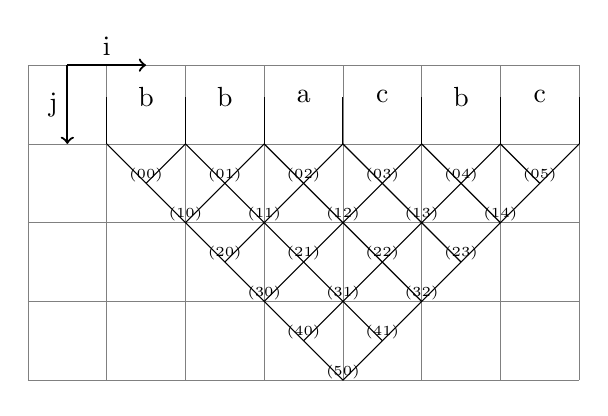
\begin{tikzpicture}[baseline]
		\newcommand{\myfontvars}[1]{
			\fontsize{4.9}{12}\selectfont{#1}
		}\newcommand{\myfontnumbering}[1]{
			\fontsize{2.5}{12}\selectfont{#1}
		}%Outer hull
		%Tip of the pyramid
		\coordinate (tip) at (3,-3);
		\foreach \i in {0,...,6} {
			\coordinate (\i) at (\i,0);
		}
		\draw[help lines] (-1,1) grid (6,-3);
		\draw [->, thick] (-0.5,1) -- (0.5,1);
		\node [above] at (0, 1) {i};
		\draw [->, thick] (-0.5,1) -- (-0.5,-0.0);
		\node [left] at (-0.5,0.5) {j};
		%Draw the left and right line of the pyramid pointing downwards
		\draw (0) -- (tip) -- (6);
		%Grid lines direction down-left to top-right
		\coordinate (dl1) at (0.5,-0.5);
		\coordinate (dl2) at (1.0,-1.0);
		\coordinate (dl3) at (1.5,-1.5);
		\coordinate (dl4) at (2.0,-2.0);
		\coordinate (dl5) at (2.5,-2.5);
		\draw (dl1) -- (1,0);
		\draw (dl2) -- (2,0);
		\draw (dl3) -- (3,0);
		\draw (dl4) -- (4,0);
		\draw (dl5) -- (5,0);
		%Grid lines direction down-right to top-left
		\coordinate (dr1) at (3.5,-2.5);
		\coordinate (dr2) at (4.0,-2.0);
		\coordinate (dr3) at (4.5,-1.5);
		\coordinate (dr4) at (5.0,-1.0);
		\coordinate (dr5) at (5.5,-0.5);
		\draw (dr1) -- (1,0);
		\draw (dr2) -- (2,0);
		\draw (dr3) -- (3,0);
		\draw (dr4) -- (4,0);
		\draw (dr5) -- (5,0);
		%Small lines at the top
		\coordinate (top0) at (0.0,0.0);
		\coordinate (top1) at (1.0,0.0);
		\coordinate (top2) at (2.0,0.0);
		\coordinate (top3) at (3.0,0.0);
		\coordinate (top4) at (4.0,0.0);
		\coordinate (top5) at (5.0,0.0);
		\coordinate (top6) at (6.0,0.0);
		\coordinate (topUpper0) at (0.0,0.6);
		\coordinate (topUpper1) at (1.0,0.6);
		\coordinate (topUpper2) at (2.0,0.6);
		\coordinate (topUpper3) at (3.0,0.6);
		\coordinate (topUpper4) at (4.0,0.6);
		\coordinate (topUpper5) at (5.0,0.6);
		\coordinate (topUpper6) at (6.0,0.6);
		\draw (top0) -- (topUpper0);
		\draw (top1) -- (topUpper1);
		\draw (top2) -- (topUpper2);
		\draw (top3) -- (topUpper3);
		\draw (top4) -- (topUpper4);
		\draw (top5) -- (topUpper5);
		\draw (top6) -- (topUpper6);
		%The string
		\coordinate (w0) at (0.5,0.6);
		\coordinate (w1) at (1.5,0.6);
		\coordinate (w2) at (2.5,0.6);
		\coordinate (w3) at (3.5,0.6);
		\coordinate (w4) at (4.5,0.6);
		\coordinate (w5) at (5.5,0.6);
		\node [] at (w0) {b};
		\node [] at (w1) {b};
		\node [] at (w2) {a};
		\node [] at (w3) {c};
		\node [] at (w4) {b};
		\node [] at (w5) {c};
		% Variables in the cells
		%cell00
		\coordinate (center00) at (0.5,0.0);
		\node [below=0.18cm] at (center00) {\myfontnumbering{$(00)$}};
		%cell01
		\coordinate (center01) at (1.5,0.0);
		\node [below=0.18cm] at (center01) {\myfontnumbering{$(01)$}};
		%cell02
		\coordinate (center02) at (2.5,0.0);
		\node [below=0.18cm] at (center02) {\myfontnumbering{$(02)$}};
		%cell03
		\coordinate (center03) at (3.5,0.0);
		\node [below=0.18cm] at (center03) {\myfontnumbering{$(03)$}};
		%cell04
		\coordinate (center04) at (4.5,0.0);
		\node [below=0.18cm] at (center04) {\myfontnumbering{$(04)$}};
		%cell05
		\coordinate (center05) at (5.5,0.0);
		\node [below=0.18cm] at (center05) {\myfontnumbering{$(05)$}};
		%cell10
		\coordinate (center10) at (1.0,-0.5);
		\node [below=0.18cm] at (center10) {\myfontnumbering{$(10)$}};
		%cell11
		\coordinate (center11) at (2.0,-0.5);
		\node [below=0.18cm] at (center11) {\myfontnumbering{$(11)$}};
		%cell12
		\coordinate (center12) at (3.0,-0.5);
		\node [below=0.18cm] at (center12) {\myfontnumbering{$(12)$}};
		%cell13
		\coordinate (center13) at (4.0,-0.5);
		\node [below=0.18cm] at (center13) {\myfontnumbering{$(13)$}};
		%cell14
		\coordinate (center14) at (5.0,-0.5);
		\node [below=0.18cm] at (center14) {\myfontnumbering{$(14)$}};
		%cell20
		\coordinate (center20) at (1.5,-1.0);
		\node [below=0.18cm] at (center20) {\myfontnumbering{$(20)$}};
		%cell21
		\coordinate (center21) at (2.5,-1.0);
		\node [below=0.18cm] at (center21) {\myfontnumbering{$(21)$}};
		%cell22
		\coordinate (center22) at (3.5,-1.0);
		\node [below=0.18cm] at (center22) {\myfontnumbering{$(22)$}};
		%cell23
		\coordinate (center23) at (4.5,-1.0);
		\node [below=0.18cm] at (center23) {\myfontnumbering{$(23)$}};
		%cell30
		\coordinate (center30) at (2.0,-1.5);
		\node [below=0.18cm] at (center30) {\myfontnumbering{$(30)$}};
		%cell31
		\coordinate (center31) at (3.0,-1.5);
		\node [below=0.18cm] at (center31) {\myfontnumbering{$(31)$}};
		%cell32
		\coordinate (center32) at (4.0,-1.5);
		\node [below=0.18cm] at (center32) {\myfontnumbering{$(32)$}};
		%cell40
		\coordinate (center40) at (2.5,-2.0);
		\node [below=0.18cm] at (center40) {\myfontnumbering{$(40)$}};
		%cell41
		\coordinate (center41) at (3.5,-2.0);
		\node [below=0.18cm] at (center41) {\myfontnumbering{$(41)$}};
		%cell50
		\coordinate (center50) at (3.0,-2.5);
		\node [below=0.18cm] at (center50) {\myfontnumbering{$(50)$}};
		\end{tikzpicture}
	}
\end{center}
\pagebreak

\begin{center}
	\resizebox{.6\linewidth}{!}{
		\begin{tikzpicture}[-,>=stealth',shorten >=1pt,auto,node distance=2cm,
		semithick]%,initial text={}]
		\tikzstyle{every state}=[fill=white,draw=black,text=black]
		
		\node     (I)            {$S1$};
		\node				(I') [below left of=I] {};
		\node (B) [left of=I']  {$A1$};
		\node (B1) [below of=B] {$c$};
		\node (C) [below right  of=I]       {$B6$};
		\node (D) [below right of=C]  {$B7$};
		\node (D2) [below left of=C]  {$C4$};
		\node (E) [below right of=D]  {$B8$};
		\node (F1) [below of=E]  {$b$};
		\node (E1) [below of=D]  {$C7$};
		\node (E3) [below of=D2]  {$C5$};
		\node (E2) [below left of=D2]  {$A2$};
		\node (F) [below  of=E1]  {$c$};
		\node (F3) [below of=E3]  {$A5$};
		\node (G1) [below  of=F3]  {$a$};
		\node (F2) [below right of=E3]  {$C6$};
		\node (G2) [below  of=F2]  {$c$};
		\node (H1) [below of=E2]  {$A3$};
		\node (H2) [below left of=E2]  {$B2$};
		\node (H3) [below left of=H2]  {$b$};
		\node (J1) [below of=H1]  {$A4$};
		\node (K1) [below of=J1]  {$a$};
		\node (J2) [below left of=H1]  {$B3$};
		\node (K3) [below of=J2]  {$b$};
		
		\path 
		(I) edge   node {$ $}   (B)
		(I) edge   node {$ $}   (C)
		(B) edge   node {$ $}   (B1)
		(C) edge   node {$ $}   (D)
		(D) edge   node {$ $}   (E)
		(C) edge   node {$ $}   (D2)
		(D2) edge   node {$ $}   (E3)
		(D) edge   node {$ $}   (E1)
		(D2) edge   node {$ $}   (E2)
		(E1) edge   node {$ $}   (F)
		(E) edge   node {$ $}   (F1)
		(E3) edge   node {$ $}   (F3)
		(E3) edge   node {$ $}   (F2)
		(F2) edge   node {$ $}   (G2)
		(F3) edge   node {$ $}   (G1)
		(E2) edge   node {$ $}   (H2)
		(E2) edge   node {$ $}   (H1)
		(H2) edge   node {$ $}   (H3)
		(H1) edge   node {$ $}   (J2)
		(H1) edge   node {$ $}   (J1)
		(J1) edge   node {$ $}   (K1)
		(J2) edge   node {$ $}   (K3)
		;
		
		\end{tikzpicture}
	}
	
\end{center}

\pagebreak
\subsection{Exam Exercise Generating Algorithms}

\subsubsection{Algorithm: AlgorithmName}
\noindent Things like the $G=(V,\Sigma , S, P)$ can be assumed as known.\\
$P = P \cup \{distribute\ \{\sigma\ |\ \sigma \in w \}\ uniform\ randomly\ over\ \{v\ |\ v \in V \} \}$ which equals the $distributeRhse$ module.\\
\noindent Bias is only allowed top vs down regarding the pyramid. No left or right bias intended yet.\\
\circled{A}, \circled{B}, ... represent exchangeable algorithm modules. Make hyperrefs für \circled{A}

\paragraph{Basic Idea}

\paragraph{Tweak Idea 1 for Algorithm}

\paragraph{Tweak Idea 2 for Algorithm}

\paragraph{Finished Algorithm}
break
\pagebreak
\subsubsection{Algorithm: GeneratorGrammarDiceRollOnly}
\noindent Very naive way of generating grammars. This is intended to be the starting point for our algorithms we find. Each found algorithm must have a higher score than this algorithm or otherwise it would be worse than simple dice rolling and then removing the useless productions.\\

\noindent
\frame{
	\begin{algorithm}[H] %or another one check
		\caption{GeneratorGrammarDiceRollOnly}
		\label{GeneratorGrammarDiceRollOnly}
		\SetAlgoLined
		\KwIn{Word $w \in \Sigma^{*}$ }
		\KwOut{Set of productions $P$}
		$P = \emptyset$;~~\tcp{$P \subseteq V \times (V^{2} \cup \Sigma)$}
		$P = Distribute(\Sigma,\ V)$;  \circled{A}\\
		$P = P \cup Distribute(V^2,\ V)$;  \circled{B}\\
		$P = P \setminus \{p\ |\ p=(v,\ x) \in P \wedge \nexists \ Cell \in Pyramid: \ v \in Cell \}$\label{useless}\;
		\Return $P$\;
		\footnotetext{
			\noindent Line \ref{useless}: Removes all useless productions. But unreachable productions still possible.
		}
	\end{algorithm}
}\\

\noindent Remove line 4 because this has nothing to do with the algorithm and write it into another procedure. In the code this is done only at the ResultCalculator.createChunkResult.

\noindent Does the output $P \subseteq V \times (V^{2} \cup \Sigma)$ imply that $G$ is in CNF? CNF does only have useful variables [TI script Def. 8.3 page 210] vs. $P \subseteq V \times (V^{2} \cup \Sigma)$.\\
\noindent More of a problem is that the set $P$ is not necessarily in CNF. It is possible that there are unreachable variables -- from the starting variable.
\pagebreak

\subsubsection{Algorithm: BottomUp GeneratorGrammarDiceRollMartens}
\noindent
\frame{
	\begin{algorithm}[H] %or another one check
		\caption{GeneratorGrammarDiceRollVar1}
		\label{GeneratorGrammarDiceRollVar1}
		\SetAlgoLined
		\KwIn{Word $w \in \Sigma^{*}$ }
		\KwOut{Set of productions $P$}
		$P = \emptyset$;~~\tcp{$P \subseteq V \times (V^{2} \cup \Sigma)$}
		$P = Distribute(\Sigma,\ V)$;  \circled{A}\\
		$Pyramid = CYK(G,\ w)$\label{stepii}\;
		\For{$i:=1\ \textbf{to}\ i_{max}$}{
			$J = \emptyset$;~~\tcp{$J \subseteq \mathbb{N}$}
			$CellSet = \emptyset$;~~\tcp{$CellSet \subseteq V^2$}
			\While{$|J| < j_{max}-i$}{
				$choose\ one\ j \notin J\ uniform\ randomly\ in\ [0, j_{max}-i] $ \label{chooseJ} \;
				$J = J \cup j$\;
				$CellSet = CalculateSubsetForCell(Pyramid,\ i,\ j)$\;
				$P = P \cup Distribute(CellSet,\ V)$;  \circled{B}\\
				$Pyramid = CYK(G,\ w)$\;	
				\If{$stopping\ criteria~met$~\circled{C}}{
					\Return $P$\;
				}
			}
		}
		\Return $P$\;
		\footnotetext{
			\noindent Line \ref{stepii}: Fills the i=0 row of the pyramid.
			
			\noindent Line \ref{chooseJ}: A cell is only visited only once.
			
			\noindent Note: Maybe modify algorithm to also work with the threshold.
		}
	\end{algorithm}
}
\\
\\
\\
Stopping criteria regarding the entire pyramid.\\

\noindent
\frame{
	\begin{algorithm}[H] %or another one check
		\caption{GeneratorGrammarDiceRollVar2}
		\label{GeneratorGrammarDiceRollVar2}
		\SetAlgoLined
		\KwIn{Word $w \in \Sigma^{*}$ }
		\KwOut{Set of productions $P$}
		$P = \emptyset$;~~\tcp{$P \subseteq V \times (V^{2} \cup \Sigma)$}
		$RowSet = \emptyset$;~~\tcp{$RowSet \subseteq \{(XY,i)\ |\ X,Y \in V \wedge i \in \mathbb{N} \}$}
		$P = Distribute(\Sigma,\ V)$;  \circled{A}\\
		$Pyramid = CYK(G,\ w)$ \label{stepii}\;
		\For{$i:=1\ \textbf{to}\ i_{max}$}{
			%$choose\ j\ uniform\ randomly\ in\ [0,\ j_{max}-i]  $\;
			\For{$j:=0\ \textbf{to}\ j_{max}-i$}{
				$RowSet = RowSet \cup \{(XY,i)\ |\ XY \in CalculateSubsetForCell(Pyramid,\ i,\ j) \}$\label{rowSet}\;
			}
			\While{$threshold_i\ not\ reached $}{
				$choose\ one~xy\ out\ of\ (XY,\ i) \in RowSet~uniform\ randomly\ with$ $probability~depending~on~i $;\label{chooseVc} \circled{D}  \\
				$P = P \cup Distribute(xy,\ V) $; \circled{B}  \\
				$Pyramid = CYK(G,\ w)$\;
				\If{$stopping\ criteria~met$~\circled{C}}{
					\Return $P$\;
				}	
			}
		}
		\Return $P$\;
		\footnotetext{
			\noindent Line \ref{stepii}: Fills the i=0 row of the pyramid.
			
			\noindent Line \ref{rowSet}: $(AB,1), (AB,2), (BC,3) ... \in sub$ $\rightarrow$ multiple occurrences of $AB$ are allowed. This considers "more important" compound variables. 
			
			\noindent Note Line \ref{chooseVc}: Priority mechanism: In line $i+1$ the $k = \{(A,l)\ |\ (A,l) \in sub,\ l=i  \}$ are preferred over the $m = \{(A,n)\ |\ (A,n) \in sub,\ n < i  \}$. In what way are they preferred? Using some kind of factor to weight the $i$ of $(A,i)$.
		}
	\end{algorithm}
}
thresholdi is regarding a line.  Threshold, Linear or log function $f(i)$?

$P = P \cup \{distribute\ vc \in rowSet\ over\ V\} $; \circled{B}  vs.\\
$P = P \cup \{distribute\ rowSet \subseteq V^2 over\ V\} $; \circled{B}  \\

(AB,3) and (AB,1) -> (AB,1)

\begin{figure}[h]
	\centering
	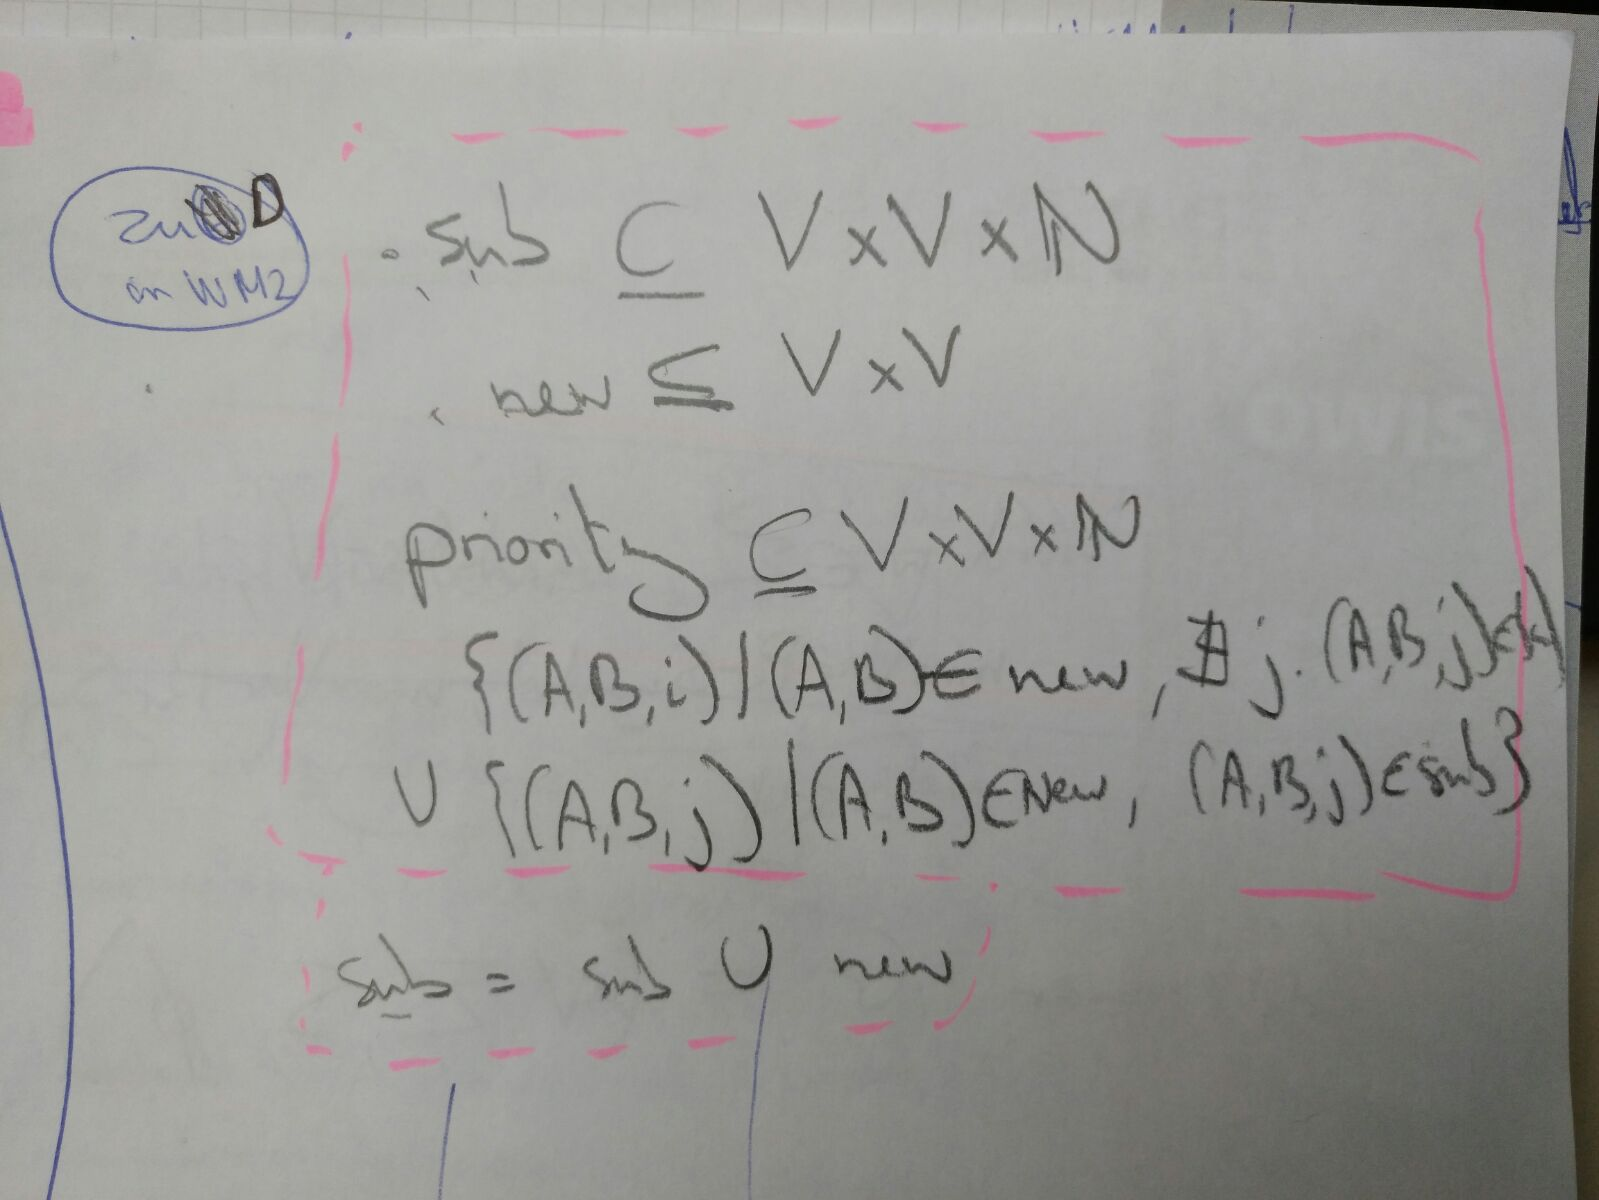
\includegraphics[width=0.7\textwidth]{abb/D_Wim2}
\end{figure}
break 
\clearpage
\newpage 


\subsubsection{Algorithm: SplitThenFill (Idea 1)}
\noindent
\frame{
	\begin{algorithm}[H] %or another one check
		\caption{SplitThenFillPrep}
		\label{SplitThenFillPrep}
		\SetAlgoLined
		\KwIn{Word $w \in \Sigma^{*}$}
		\KwOut{Set of productions $P$}
		$P = \emptyset$;~~\tcp{$P \subseteq V \times (V^{2} \cup \Sigma)$}
		$P = Distribute(\Sigma,\ V)$; \circled{A} \label{stepii}  \\		
		$Sol = \emptyset$;~~\tcp{$Sol \subseteq \{(P_{Sol},~Cell_{i,j})~|~P_{Sol} \subseteq P \wedge Cell_{i,j} \in Pyramid\}$} \label{cell}
		$Sol = SplitThenFill(P,\ w,\ i_{max},\ 0)$\;
		\Return $P_{Sol}$\;
		\footnotetext{
			\noindent Line \ref{stepii}: Fills the i=0 row of the pyramid.	
					
			\noindent Line \ref{cell?}: $Cell_{i,j} \subseteq V \wedge Cell_{i,j} \in Pyramid$. The pyramid represents the upper part of the upper triangular matrix of the CYK. Reflection at the diagonal of the matrix and rotation of -45 degrees.
			
			\noindent Line \ref{tip2}: Starting recursively from the tip of the pyramid.
		}
	\end{algorithm}
}
\\

\noindent
\frame{
	\begin{algorithm}[H] %or another one check
		\caption{SplitThenFill}
		\label{SplitThenFill}
		\SetAlgoLined
		\KwIn{$P \subseteq V \times (V^{2} \cup \Sigma),\ w \in \Sigma^{*},\ i,j \in \mathbb{N}$ }
		\KwOut{$(P,~Cell_{i,j})$}
		\If{$i=0$}{
			\Return $(P,\ Cell_{i,j})$\label{row0}\;
		}
		\If{$stopping\ criteria~met$~\circled{C}}{
			\Return $(P,\ Cell_{i,j})$\;
		}	
		$choose\ one\ m\ uniform\ randomly\ in\ [j+1,\ j+i]$\;
		$(P,\ Cell_l) = SplitThenFill(P,\ w,\ (m-j-1),\ j)$\label{left}\;
		$(P,\ Cell_r) = SplitThenFill(P,\ w,\ (j+i-m),\ m)$\label{right}\;
		$Pyramid = CYK(G,\ w)$\label{cyk}\;
		\If{$Cell_{i,j} = \emptyset$}{
			$SetVc = uniform\ random\ subset\ from\ \{vc\ |\ v \in Cell_l\ \wedge\ c \in Cell_r\}$\;
			$P = P \cup Distribute(SetVc,\ V) $; \circled{B}  \\
		}
		
		\Return $(P,\ Cell_{i,j})$\;
		\footnotetext{
			\noindent Line \ref{row0}: Recursion anchor that returns the up to this point modified productions $P$ and the variables in the cell with index i and j. 
			
			\noindent Line \ref{left} + \ref{right}: Analogous to the CYK-algorithm a cell combination $Cell_l$ and $Cell_r$ is chosen that can generate the sub string. 
			
			\noindent Line \ref{cyk}: A Recalculation is done at each recursive call because only the updated production set $P$ is returned recursively.
		}
	\end{algorithm}
}
\\
\\
The stopping criteria would be, that each marked $cell_{i,j} \neq \emptyset$ and it must be possible to get from $cell_{m, j}$ and $cell_{i-m, m+j+1}$ to $cell_{i,j}$ through applying one of the production rules.\\
Algorithm \ref{Idea1} Idea1 uniform randomly generates a predefined structure of the derivation tree. You always update the pyramid after adding one production to the grammar. Now there are two options to fill the parse table:
\begin{enumerate}
	\item Bottom Up: The parse table is filled relatively evenly. All information regarding the upper cells are available and can be used. Similar to the CYK Algorithm approach.
	\item Top Down: The parse table is filled quiet unevenly. You don't have all information available. Think about adding a production for the node cell: You can add a production so that its producing cells fill the node cell, but you don't know what actually would be the best to fill in these producing cells because they themselves aren't looked at yet. This problem is kept until the last depth of the recursion, where the cells in row $i=0$ are taken into account. Only starting there you know what variables actually produce the terminals.\\
	Maybe solution: For the Top Down approach, don't assume that the terminals are already distributed over the V. Distribute the terminals over the variables in an ideal way that fits your already generated productions best.
\end{enumerate}

\pagebreak

\subsubsection{Algorithm: Idea 2, How often cells are used for subset calculations}

\pagebreak

\subsubsection{Algorithm: SplitAndFill}
\noindent
\frame{
	\begin{algorithm}[H] %or another one check
		\caption{SplitAndFillPrep}
		\label{SplitAndFillPrep}
		\SetAlgoLined
		\KwIn{Word $w \in \Sigma^{*}$}
		\KwOut{Set of productions $P$}
		$P = \emptyset$;~~\tcp{$P \subseteq V \times (V^{2} \cup \Sigma)$}
		$Pyr = EmptyPyramid$ \label{emptyPyramid}\;
		$Cell_{i_{max},0} = Cell_{i_{max},0} \cup \{S\}$;~~\tcp{$Cell_{i,j} \subseteq V \wedge Cell_{i,j} \in Pyramid$} \label{cell}
		\;
		$Sol = \emptyset$;~~\tcp{$Sol \subseteq \{(P_{Sol},~Pyramid)~|~P_{Sol} \subseteq P$\}} \label{cell}	
		$Sol = SplitThenFill(Pyr,\ P,\ w,\ i_{max},\ 0)$\;
		$P = P \cup P_{Sol}$\; \label{tip}
		\Return $P$\;
		\footnotetext{
			\noindent Line \ref{emptyPyramid}: $EmptyPyramid \Leftrightarrow \forall i\ \forall j\ Cell_{i,j}=\emptyset$
			
			\noindent Line \ref{cell}: $Cell_{i,j} \subseteq V \wedge Cell_{i,j} \in Pyramid$. The pyramid represents the upper part of the upper triangular matrix of the CYK. Reflection at the diagonal of the matrix and rotation of -45 degrees.
		}
	\end{algorithm}
}
\\

\noindent
\frame{
	\begin{algorithm}[H] %or another one check
		\caption{SplitAndFill}
		\label{SplitAndFill}
		\SetAlgoLined
		\KwIn{$Pyramid~Pyr,\ P \subseteq V \times (V^{2} \cup \Sigma),\ w \in \Sigma^{*},\ i,j \in \mathbb{N}$ }
		\KwOut{$(P,~Pyr)$}
		\If{$stopping\ criteria~met$~\circled{C}}{
			\Return $(P,\ Pyr)$\;
		}
		$SetAll = V \times V$\;
		$Pyramid = CYK(G,\ w)$\label{cyk}\;
		$choose\ one\ m\ uniform\ randomly\ in\ [j+1,\ j+i]$\;
		
		\If{$(m-j-i) \neq 0$}{
			$(P,\ Pyr) = SplitAndFill(Pyr,\ w,\ (m-j-1),\ j)$\label{left}\;	
		} else then\\
			~~~~~~$v = choose~one~variable~uniform~randomly~from~Cell_{i,j}$\;
			~~~~~~$P = P \cup (v --> w_j)$\;
		end
		
		\If{$(j+i-m) \neq 0$}{
			$(P,\ Pyr) = SplitAndFill(Pyr,\ w,\ (j+i-m),\ m)$\label{right}\;
		} else then\\
			~~~~~~$v = choose~one~variable~uniform~randomly~from~Cell_{i,j}$\;
			~~~~~~$P = P \cup (v --> w_j)$\;
		end
		\Return $(P,\ Cell_{i,j})$\;
		\footnotetext{
		}
	\end{algorithm}
}
\\

\pagebreak

\subsubsection{Tweaking Sub Procedures in more detail}
Maybe don't keep this so that the Algorithms can be read without flipping pages.\\
$\circled{A}, \circled{B}, ...$\\
\noindent
\frame{
	\begin{algorithm}[H] %or another one check
		\caption{Distribute}
		\label{Distribute}
		\SetAlgoLined
		\KwIn{ $Rhse \subseteq\ (V^{2} \cup \Sigma),\ V$}
		\KwOut{Set of productions $P$}
		$i \in  \mathbb{N},\ j \in  \mathbb{N}$\;
		\ForEach{$rhse \in Rhse$}{
			$choose\ n\ uniform\ randomly\ in\ [i, j]$\;
			$V_{add} := uniform\ random\ subset\ of\ size\ n\ from\ V$\;
			$P = P \cup \{ (v, rhse)\ |\ v \in V_{add},\ rhse \in Rhse \} $\;	
		}
		\Return $P$;
	\end{algorithm}
}
Algorithm \ref{Distribute} isn't needed anymore for the descriptions of the basic idea of the algorithm. It will be a module later on while tweaking the algorithms.
\\
\\
\frame{
	\begin{algorithm}[H] %or another one check
		\caption{CalculateSubsetForCell}
		\label{CalculateSubsetForCell}
		\SetAlgoLined
		\KwIn{$cell_ {i,j} \in pyramid $}
		\KwOut{$V_{i,j} \subseteq V^2$}
		$V_{i,j} = \emptyset $\;
		\For{$k:=i-1 \to 0$}{
			$V_{i,j} = V_{i,j} \cup \{X\ |\ X\longrightarrow YZ,\ Y \in V_{k,j},\ Z \in V_{i-k-1,k+j+1} \}$\;
		}
		
		\Return $V_{i,j}$\;
	\end{algorithm}
}
Algorithm \ref{calculateSubsetForCell} describes the magic of the CKY-algorithm. It shows what cells are taken into account while filling one cell of the parse table.

\pagebreak

\subsection{Criteria Checking Procedures}
\noindent Description of the checks here. \\
\noindent All test of the GrammarValidityChecker class are based on the simple setV matrix. \\

\noindent  isValid = isWordProducible \&\& isExamConstraints \&\& isGrammarRestrictions\\

\noindent  isWordProducible = CYK.algorithmAdvanced()\\

\noindent  isExamConstraints = isRightCellCombinationsForced \&\& isMaxSumOfProductionsCount \&\& isMaxSumOfVarsInPyramidCount \&\& countRightCellCombinationsForced \\

\noindent isGrammarRestrictions = isSizeOfWordCount \&\& isMaxNumberOfVarsPerCellCount \\
\\
\\
\noindent 
\frame{
	\begin{algorithm}[H] %or another one check
		\caption{checkForceCombinationPerCell}
		\label{checkRightCellPerCombination}
		\SetAlgoLined
		\KwIn{$ cell_{i,j}\subseteq V,\ cell_{i-1,j}\subseteq V,\ cell_{i-1,j+1} \subseteq V,\ P \subseteq V \times (V^{2} \cup \Sigma) $ }
		\KwOut{$varsForcing \subseteq V$}
		$varsForcing \subseteq V$\;
		$varComp = \{XY\ |\ X \in cell_{i-1,j}\ \wedge\ Y \in cell_{i-1,j+1} \}$\;
		\ForEach{$v \in cell_{i,j}$}{
			$prods = \{p\ |\ p \subseteq P,\ v\ is\ left\ in\ p \}$\;
			$rhses = \{rhse\ |\ rhse\ is\ right\ in\ p \in prods\} $\;
			\If{$varComp \nsubseteq rhses$}{
				$varsForcing = varsForcing \cup v$\;
			}			
		}
		\Return $varsForcing$\;
		\footnotetext{Input: $cell_{i,j} = cellDown$, $cell_{i-1,j} = cellUpperLeft$ and $cell_{i-1,j+1} = cellUpperRight$
		}
	\end{algorithm}
}
Algorithm \ref{checkRightCellPerCombination} is a check that needs to be explained.
\\
\\
\frame{
	\begin{algorithm}[H] %or another one check
		\caption{checksumOfProductions}
		\label{checksumOfProductions}
		\SetAlgoLined
		\KwIn{$ max \in \mathbb{N}_{\geq 0}  $ }
		\KwOut{$ true \iff sum \leq max$}
		\If{$|P| > max $}{
			\Return $fales$\;
		}
		\Return $true$\;
	\end{algorithm}
}
Algorithm \ref{checksumOfProductions} can be explained via the Output of the algorithm alone.

\pagebreak

\noindent
\frame{
	\begin{algorithm}[H] %or another one check
		\caption{checkMaxNumberOfVarsPerCell}
		\label{checkMaxNumberOfVarsPerCell}
		\SetAlgoLined
		\KwIn{$ max \in \mathbb{N}_{\geq 0}  $ }
		\KwOut{$ true \iff \forall cell_{i,j} \in pyramid,\ |cell_{i,j}| \leq max $}
		\For{$i:=1\ \textbf{to}\ i_{max}$}{
			%$choose\ j\ uniform\ randomly\ in\ [0,\ j_{max}-i]  $\;
			\For{$j:=0\ \textbf{to}\ j_{max}-i$}{
				\If{$|cell_{i,j}| > max$}{
					\Return $false$\;
				}
			}
		}
		\Return $true$\;
	\end{algorithm}
}
Algorithm \ref{checkMaxNumberOfVarsPerCell} can be explained via the Output of the algorithm alone.
\\
\\
\noindent
\frame{
	\begin{algorithm}[H] %or another one check
		\caption{checkMaxSumOfVarsInPyramid}
		\label{checkMaxSumOfVarsInPyramid}
		\SetAlgoLined
		\KwIn{$ max \in \mathbb{N}_{\geq 0}  $ }
		\KwOut{$ true \iff sum \leq max $}
		$sum = 0$\;
		\For{$i:=1\ \textbf{to}\ i_{max}$}{
			%$choose\ j\ uniform\ randomly\ in\ [0,\ j_{max}-i]  $\;
			\For{$j:=0\ \textbf{to}\ j_{max}-i$}{
				$sum = sum + |cell_{i,j}|$\;
				\If{$sum > max$}{
					\Return $false$\;
				}
			}
		}
		\Return $true$\;
	\end{algorithm}
}
Algorithm \ref{checkMaxSumOfVarsInPyramid} could possible be explained via a simple mathematical statement like the algorithms \ref{checksumOfProductions} and \ref{checkMaxNumberOfVarsPerCell}.

\pagebreak